\section{Resolución Problema 4}

\subsection{\textbf{INTRODUCCIÓN} } 

El sistema binario es un sistema numérico que se compone únicamente de dos dígitos, 0 y 1, utilizados para representar valores. La conversión de números decimales (base 10) a números binarios (base 2) . El propósito de este proyecto es desarrollar un algoritmo eficiente para convertir números decimales enteros, tanto positivos como negativos, a su equivalente binario.

La metodología para convertir un número decimal entero a binario implica dividir de forma sucesiva el número decimal entre 2 y registrar el residuo de cada división. Estos residuos son  leídos de abajo hacia arriba y conformarán el número binario equivalente. En el caso de números negativos, se utiliza el complemento a dos para representar tanto el signo como el valor absoluto del número.


El resultado del  algoritmo desarrollado se va a demostrar ser  preciso y eficiente en la conversión de números decimales enteros a binarios. A través de pruebas y verificaciones, el algoritmo proporcionara resultados correctos y coherentes para distintos valores de entrada. Esto permitirá una conversión confiable y precisa de números decimales enteros a binarios, lo cual resultara fundamental en diversas aplicaciones.


\subsection{\textbf{Descripción del problema:}}

\subsection{\textbf{DESCRIPCIÓN DEL PROBLEMA} } 
Implica comprender y definir claramente el problema que se quiere resolver. En este caso, se trata de convertir un número decimal a binario.


\begin{figure}[h!]
    \centering
    \includegraphics[width = 6 cm]{LaTeX/latex-imagenes/DECIMAL.png}
    \caption{Decimal a binario}
    \label{decimal a binario}
\end{figure}


\subsection{\textbf{Definición de solución:}}

\subsection{\textbf{DEFINICIÓN DE SOLUCIÓN} }
En esta etapa, se determina el enfoque o algoritmo general que se utilizará para convertir el número decimal a binario. 


%diagrama
\begin{figure}[H]
\centering
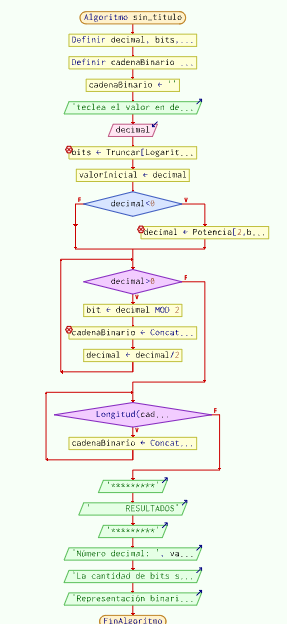
\includegraphics[width=6cm]{LaTeX/latex-imagenes/1.png}
\caption{Diagrama de flujo que muestra el proceso para resolver }
\label{fig:diagrama_flujo}

\end{figure}


\subsection{\textbf{Diseño de la solución:}}

\subsection{\textbf{DISEÑO DE SOLUCIÓN} }
\subsection{\textbf{\textit{Programa en Java}}}
Se detallan los pasos específicos y la lógica necesaria para implementar el algoritmo definido anteriormente. Se pueden utilizar diagramas, pseudocódigo u otras herramientas para representar visualmente el flujo de la solución.

\subsectionse \textit{\textbf{solicita al usuario que teclee el valor decimal}}

\begin{lstlisting}[style=javaStyle]
package com.mycompany.programacorrecto;

import java.util.Scanner;

/**MARCO ANTONIO MENDOZA CALVA
 */
 public class Programacorrecto {

    public static void main(String[] args) {
     Scanner h=new Scanner(System.in);
     System.out.println("Teclea el valor en decimal : ");
\end{lstlisting}
**
%codigo
\subsectionse\textbf{\textit{calcula los bits del numero entero que dio el usuario}}

\begin{lstlisting}[style=javaStyle]
int decimal=h.nextInt();
     int bits = (int) (Math.log(Math.abs(decimal)) / 
     Math.log(2)) + 1;//calcular los bits del numero entero.
\end{lstlisting}

\subsectionse\textbf{\textit{Verificar si el número es negativo (-)}}

\begin{lstlisting}[style=javaStyle]
        int valorinicial=decimal;    
    
       
        // Verificar si el número es negativo (-)
        if (decimal < 0) {
\end{lstlisting}

\subsectionse\textbf{\textit{Obtener la representación en complemento a 2}}

\begin{lstlisting}[style=javaStyle]
  // Obtener la representación en complemento a 2
            decimal = (int) (Math.pow(2, bits) + decimal);
        }
\end{lstlisting}
\subsectionse\textbf{\textit{Convertir Numero decimal a binario}}

\begin{lstlisting}[style=javaStyle]
  // Convertir Numero decimal a binario
        StringBuilder binary = new StringBuilder();
        do {
\end{lstlisting}


\subsectionse\textbf{\textit{Obtener el bit menos significativo}}

\begin{lstlisting}[style=javaStyle]
  // Obtener el bit menos significativo
            int bit = decimal % 2;
\end{lstlisting}
\subsectionse\textbf{\textit{Agregar el bit al inicio de la cadena}}

\begin{lstlisting}[style=javaStyle]
  // Agregar el bit al inicio de la cadena
            binary.insert(0, bit);

\end{lstlisting}

\subsectionse\textbf{\textit{Dividir el número por 2}}

\begin{lstlisting}[style=javaStyle]
   // Dividir el número por 2
            decimal /= 2;
        } while (decimal > 0);

\end{lstlisting}

\subsectionse\textbf{\textit{Ajustar la longitud al número de bits especificado}}

\begin{lstlisting}[style=javaStyle]
    // Ajustar la longitud al número de bits especificado
        while (binary.length() < bits) {
            binary.insert(0, '0');
        }

\end{lstlisting}

\subsectionse\textbf{\textit{converitr a cadena}}

\begin{lstlisting}[style=javaStyle]
    String binario =binary.toString(); //

\end{lstlisting}
\subsectionse\textbf{\textit{final mente se obtienen los resultados}}

\begin{lstlisting}[style=javaStyle]
     System.out. println("       RESULTADOS    ");
        System.out.println("El Número decimal es : \t" + valorinicial);
        System.out. println("La cantidad de bits son: \t "+ bits);
        System.out.println("El numero binario es :\t " + binario);
    }       
}

\end{lstlisting}


\subsection{\textbf{Desarrollo de la solución:}}

\subsection{\textbf{DESARROLLO DE SOLUCIÓN }}
Implementa el algoritmo utilizando un lenguaje de programación específico. Se escriben líneas de código que siguen la lógica y los pasos definidos en la etapa de diseño. Es importante asegurarse de que el código sea claro, legible y esté correctamente estructurado.
\subsection{\textbf{Código completo}}
\begin{lstlisting}[style=javaStyle]
package com.mycompany.programacorrecto;

import java.util.Scanner;

/**MENDOZA CALVA MARCO ANTONIO

 */
public class Programacorrecto {

    public static void main(String[] args) {
     Scanner h=new Scanner(System.in);
     System.out.println("Teclea el valor en decimal : ");
     int decimal=h.nextInt();
     int bits = (int) (Math.log(Math.abs(decimal)) / Math.log(2)) + 1;//calcular los bits del numero entero.
     int valorinicial=decimal;    
    
       
        // Verificar si el número es negativo (-)
        if (decimal < 0) {
            // Obtener la representación en complemento a 2
            decimal = (int) (Math.pow(2, bits) + decimal);
        }

        // Convertir Numero decimal a binario
        StringBuilder binary = new StringBuilder();
        do {
            // Obtener el bit menos significativo
            int bit = decimal % 2;
            // Agregar el bit al inicio de la cadena
            binary.insert(0, bit);
            // Dividir el número por 2
            decimal /= 2;
        } while (decimal > 0);

        // Ajustar la longitud al número de bits especificado
        while (binary.length() < bits) {
            binary.insert(0, '0');
        }

        
        String binario =binary.toString(); //converitr a cadena 
        System.out. println("       RESULTADOS    ");
        System.out.println("El Número decimal es : \t" + valorinicial);
        System.out. println("La cantidad de bits son: \t "+ bits);
        System.out.println("El numero binario es :\t " + binario);
    }       
}

\end{lstlisting}


\subsection{\textbf{Depuración y pruebas:}}

\subsection{\textbf{DEPURACIÓN Y PRUEBAS} }
 verifica y corrige cualquier error que pueda existir en el código. Se realizan pruebas exhaustivas utilizando diferentes casos de prueba, incluyendo números decimales enteros positivos y negativos, para garantizar que la conversión a binario funcione correctamente en todos los escenarios posibles.

 \begin{figure}[h!]
    \centering
    \includegraphics[width = 6 cm]{LaTeX/latex-imagenes/PRUEBA.png}
    \caption{ CORRIDA}
    \label{codigo de java }
\end{figure}

\begin{figure}[h!]
    \centering
    \includegraphics[width = 6 cm]{LaTeX/latex-imagenes/tabla.png}
    \caption{ TABLA DE CORRIDAS }
    \label{codigo de java }
\end{figure}
\vspace*{-8pt}